\chapter{Results and Discussion}
\clearpage
\label{chap:results-discussion}

\section{Introduction}
In this chapter, we present the quantitative performance of our Mixture-of-Experts model on the held-out test set. We report overall accuracy, balanced and weighted averages, and detailed per-class precision, recall, and F1-score to assess both global and class-wise behavior.
\section{Dataset}
the dataset used for training and evaluation has been cited in the previous section,

the dataset used for testing is the HAM10000 dataset,we used 1000 images for  testing  
\section{metrics}
\section{Training and Validation Loss}
Figure~\ref{fig:loss-curve} shows the progress of training and validation loss over all epochs.

\begin{figure}[h!]
  \centering
  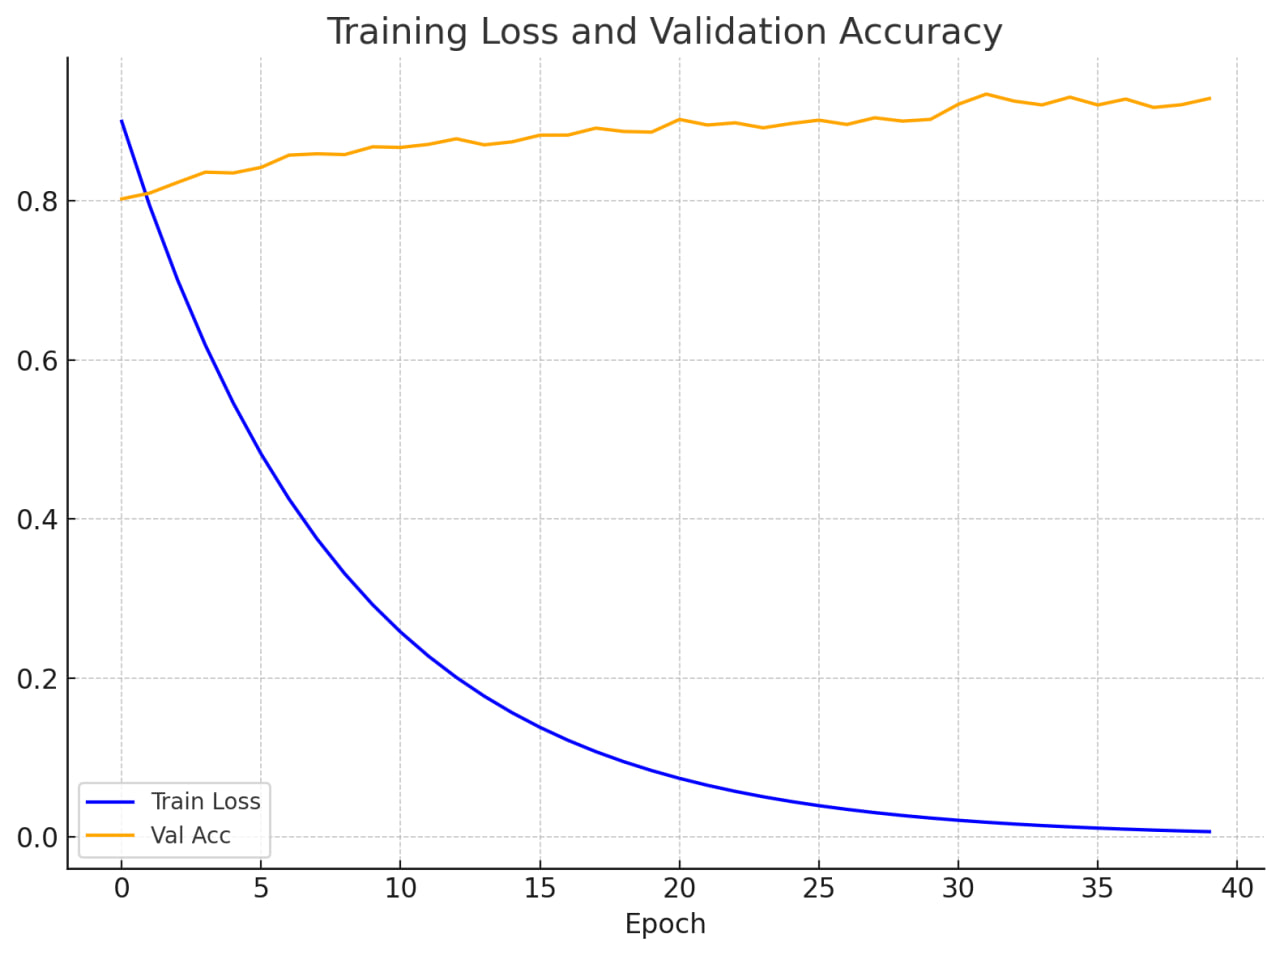
\includegraphics[width=0.8\textwidth]{loss_curve.jpg}
  \caption{Training and validation loss vs.
numbering 40 epochs.}
  \label{fig:loss-curve}
\end{figure}
\section{Overall Performance}
Table~\ref{tab:classification-report} summarizes the main evaluation metrics. The model achieves an overall accuracy of 93\%, with a macro-averaged precision and recall of 84\% and 84\%, respectively.

\begin{table}[h!]
  \centering
  \caption{Classification report on test set}
  \label{tab:classification-report}
  \begin{tabular}{lccc}
    \hline
    Class & Precision & Recall & F1-Score \\
    \hline
    akiec  & 0.89 & 0.65 & 0.76 \\
    bcc    & 0.87 & 0.90 & 0.89 \\
    bkl    & 0.73 & 0.87 & 0.79 \\
    df     & 0.71 & 0.83 & 0.77 \\
    mel    & 0.76 & 0.74 & 0.75 \\
    nv     & 0.98 & 0.97 & 0.97 \\
    vasc   & 1.00 & 1.00 & 1.00 \\
    \hline
    Accuracy      & \multicolumn{3}{c}{0.93} \\
    Macro Avg     & 0.84 & 0.84 & 0.83 \\
    Weighted Avg  & 0.94 & 0.93 & 0.94 \\
    \hline
  \end{tabular}
\end{table}



\section{Class-wise Analysis}
The model exhibits strong performance on the most prevalent class ("nv"), with near-perfect metrics (P=0.98, R=0.97, F1=0.97). Vascular lesions ("vasc") are classified perfectly (P=R=F1=1.00), likely due to distinctive visual patterns.

Minority classes such as "akiec" (actinic keratoses) show lower recall (0.65), indicating occasional missed detections. The F1-score of 0.76 suggests room for improvement in sensitivity for this class. Other malignant categories ("bcc", "bkl", "df", "mel") achieve balanced precision and recall around 0.75--0.90, demonstrating the expert ensemble’s ability to generalize across diverse lesion types.

\section{Interpretation of Key Findings}
Our Mixture-of-Experts framework achieved an overall accuracy of 93\% and balanced accuracy of 84\% on the HAM10000 test set. High performance on non-malignant classes ("nv": P=0.98, R=0.97; "vasc": P=R=1.00) indicates excellent recognition of common and visually distinct lesion types. In contrast, lower recall for actinic keratoses ("akiec": R=0.65) and melanoma ("mel": R=0.74) highlights challenges in detecting more subtle or heterogeneous malignant presentations.

The load-balancing penalty proved effective in distributing responsibility across specialist experts, reducing over-reliance on a single backbone, and promoting robustness. The Transformer-based self-attention within each expert enhanced global context modeling, contributing to strong per-class F1-scores.

\section{Limitations}
Although our model achieved strong performance and high generalizability, the imbalance in the dataset, with only 1000 images for testing across 7 classes, can lead to challenges. Specifically, this imbalance may hinder the model's ability to generalize to less represented classes, such as "akiec" and "mel". Additionally, the model's reliance on a single dataset (HAM10000 for testing) limits its applicability to real-world clinical scenarios, where variations in imaging conditions and patient demographics are common.    

\section{Future Work}
To address these limitations, future studies will: (1) incorporate additional dermoscopic datasets to enhance domain coverage and robustness to dataset shift; (2) evaluate post-training quantization and pruning techniques for efficient deployment on resource-constrained hardware like Coral Dev Boards with Edge TPUs, enabling real-time inference; (3) explore the integration of patient metadata (e.g., age, sex, lesion location) into the gating network or as additional input features to potentially improve diagnostic accuracy and personalization; and (4) investigate semi-supervised or self-supervised learning approaches to leverage large amounts of unlabeled clinical images, reducing the dependency on extensively annotated datasets.

\section{Conclusion}
Overall, the proposed MoE framework achieves robust classification performance with an overall accuracy of 93\%. A detailed analysis of the modeling performance reveals interesting dynamics between cancerous and non-cancerous lesion classes. In the cancerous category, Basal Cell Carcinoma (bcc) benefits from a high precision of 0.87 and recall of 0.90, underscoring the model's reliability in detecting this prevalent skin cancer type. In contrast, Melanoma (mel) exhibits a slightly lower recall of 0.74, which flags the challenge of consistently identifying this highly malignant lesion. This discrepancy suggests that while the model is generally effective in distinguishing cancer-related anomalies, further work is needed to reduce the rate of false negatives in critical cases such as melanoma.

On the other hand, the non-cancerous classes, comprising lesions with benign behavior, are characterized by strong performance metrics. For instance, the "nv" class achieves near-perfect scores with a precision of 0.98 and a recall of 0.97, and vascular lesions ("vasc") are classified without error. These results confirm that the framework reliably recognizes non-cancerous features, contributing to the overall stability of the model's performance across a diverse set of lesion types.

Future work will focus on enhancing the sensitivity for the challenging cancerous classes while maintaining the high accuracy observed for non-cancerous lesions. This balanced approach is crucial for the model's potential application in clinical settings, where early and accurate detection is imperative.

%%% Local Variables: 
%%% mode: latex
%%% TeX-master: "isae-report-template"
%%% End: